% !TEX root = BA-Bauer

\subsection{Schaltungsprinzip}

In diesem Kapitel wird auf das grundlegende Prinzip der gesamten Schaltung eingegangen. Auf die einzelnen Komponenten und deren benötigte Beschaltung wird in den folgenden Kapiteln eingegangen. Generell wird bei der Entwicklung der Schaltung darauf geachtet, dass möglichst keine fertigen Modulbausteine verwendet werden. Dadurch ergibt sich in der Regel ein Preisvorteil und vereinfacht die industrielle Bestückung der Platine, in Hinsicht auf eine Serienproduktion. %(Quelle?)
Abbildung \ref{fig:Schaltungsrinzip} zeigt das grundlegende Prinzip der Schaltung. Auf der linken Seite befindet der Benutzer des Gerätes. Er bedient das Gerät durch seine Eingaben und erhält entsprechende Rückmeldungen zurück. Die grüne Fläche spiegelt das Gerät wieder, welches mit der DMX-Quelle bzw. der DMX-fähigen Lichttechnik auf der rechten Seite kommuniziert. Im Folgenden wird auf die Bestandteile des Gerätes eingegangen.
\begin{figure}[h]
	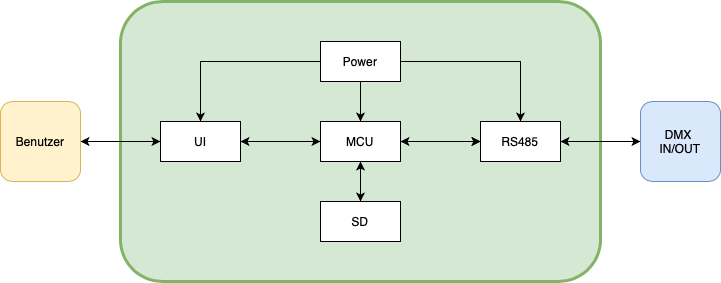
\includegraphics[width = \textwidth]{Schaltungsprinzip}
	\caption{Schaltungsprinzip}
	\label{fig:Schaltungsrinzip}
\end{figure}\\
\textbf{Mikrocontroller (MCU)}\\
Der Mikrocontroller, im Folgenden MCU genannt, bildet den Mittelpunkt der Schaltung. Die auf ihm ausgeführte Software steuert die Benutzerschnittstelle (UI), speichert und ruft Daten vom Speicher ab und sendet und empfängt die DMX-Daten. Aufgrund der hohen Anforderungen an den MCU wird bei der Entwicklung ein besonderes Augenmerk auf ihn und seine Beschaltung gelegt. Die Auswahl des MCUs orientiert sich an dem in der Praxisprojektarbeit verwendeten Mikrocontroller, da dessen Funktionsfähigkeit bereits erwiesen ist.\\
\newline
\textbf{Spannungsversorgung (Power)}\\
Alle Komponenten werden von einer USB-Schnittstelle mit Spannung versorgt. Da das Gerät eigenständig verwendet werden soll, werden über die Schnittstelle keine Daten übertragen. Die Schnittstelle liefert 5\,V Spannung \cite[S. 44]{USB-Battery}, welche in die benötigten Spannungen transformiert wird. Besonders kritisch ist die Spannungsversorgung des MCUs, denn unter normalen Betriebsbedingungen darf die Versorgungsspannung nur soweit einbrechen, dass der MCU weiterhin den darauf befindlichen Programmcode fehlerfrei ausführen kann.\\
\textbf{Benutzerschnittstelle (UI)}\\
Damit der Benutzer das Gerät bedienen kann, ist ein Informationsfluss in zwei Richtungen erforderlich. Zum Einen müssen Eingaben durch den Benutzer erfasst werden, zum Anderen muss das Gerät dem Benutzer eine Rückmeldung über Fehler oder den aktuellen Status geben können. Für die Benutzereingaben werden mehrere Taster und ein Drehgeber (Encoder) verwendet. Durch den Einsatz von Tastern können präzise und zeitgenaue Eingaben vom Benutzer vorgenommen werden, an Stellen an denen es nötig ist, zum Beispiel beim Starten einer Wiedergabe. Der Encoder hingegen bietet die Möglichkeit viele Eingaben in kurzer Zeit zu tätigen, zum Beispiel beim Einstellen der Aufnahmezeit. Für die Ausgaben werden mehrere LEDs und ein Display verwendet.\\
\newline
\textbf{RS485}\\
Die RS485-Schnittstelle ist die Verbindung zwischen DMX-Quelle/Senke und dem MCU. Diese ist notwendig ist, da der MCU keine RS485 konformen Signalpegel liefern, oder auswerten kann. Zudem werden durch die Schnittstelle die DMX-Leitungen galvanisch von der restlichen Schaltung getrennt. Spannungs- und Stromspitzen ausgehend von den DMX-Leitungen können so die Schaltung nicht beeinträchtigen oder beschädigen.\\
\newline
\textbf{Speicher (SD-Karte)}\\
Damit ein sinnvoller Einsatz des Gerätes möglich ist, müssen die aufgenommenen Daten auch nach einem Neustart des Geräts verfügbar sein. Deswegen ist die Sicherung der Daten auf einem Speichermedium notwendig. In der vorangegangen Praxisprojektarbeit wurde bereits gezeigt, dass der Einsatz einer SD-Karte für diesen Zweck geeignet ist. Die Verwendung einer SD-Karte ermöglicht dem Benutzer außerdem eine gewisse Sicherheit in Bezug auf den Schutz der Daten. Eine Sicherungskopie der Daten kann einfach auf einem PC erstellt werden. Zudem können für verschiedene Einsatzgebiete verschiedene SD-Karten verwendet werden.